\chapter{Setup of JICF gaseous inlet profile}
\label{app:JICF_BL_setup}

This appendix describes the mathematical derivations to impose a gaseous inlet velocity profile in the JICF simulations presented in Chapter \ref{ch5:jicf_resolved_simulations}. The modeled geometry representing the experimental test bench is shown in Figure \ref{fig:numerical_setup_maquette_JICF_DLR}. The gaseous inlet consists of a rectangular channel of section 25x40 mm$^2$. The experiments \citepColor[becker_breakup_2002] report a gaseous boundary layer thickness $\delta_\mathrm{exp}$ of between 4 and 5 mm at the lip of the liquid injector, so a profile aiming at obtaining this thickness is developed. The computational domain of the JICF (Figure \ref{fig:numerical_setup_maquette_JICF_DLR}) is a reduced portion of the experimental test rig (Figure \ref{fig:experiment_JICF_DLR}), so an artificial velocity profile with a boundary layer is imposed at the gaseus inlet. The gaseous inlet boundary and the repartition performed to impose boundary layer profiles is shown in Figure \ref{fig:domain_partition_3D_profile}.


\begin{figure}[h!]	
	\centering
	\includeinkscape[inkscapelatex=true,width=13cm]{./appendices_figures/domain_partition}
%	\includesvg[width=13cm,pretex=\normalsize,svgpath=./files/Images/3D_BL/]{domain_partition}
	\caption{Inlet domain and partition into sections for calculation of the gaseous velocity profile in JICF simulations}
	\label{fig:domain_partition_3D_profile}
\end{figure}



Due to symmetry in both $y$ and $z$ directions, only one fourth of the domain is considered to derive the equations. In this part of the domain, the volumetric flow rate given by the bulk velocity $u_g$ is the following one:

\begin{equation}
\label{eq:volumetric_flow_rate_2D}
Q = u_g b_y b_z
\end{equation}	

where $b_y = 25/2 = 12.5$ mm and $b_z = 40/2 = 20$ mm, so the total volumetric flow rate is $4Q$ which agrees with the volumetric flow rate shown in Table \ref{tab:jicf_operating_conditions}. For deriving the equations, the domain is divided in 4 sections as shown in Figure \ref{fig:domain_partition_3D_profile}, where different profiles are imposed:

\begin{enumerate}

	\item Section 1 (\textbf{S1}): Boundary layer profile in both lateral ($y$) and vertical ($z$) directions.
	
	\item Section 2 (\textbf{S2}): Boundary layer profile in $y$; outer, constant velocity in $z$.
	
	\item Section 3 (\textbf{S3}): Outer, constant velocity in $y$; boundary layer profile in $z$.
	
	\item Section 4 (\textbf{S4}): Outer, constant velocity in both $y$ and $z$.

\end{enumerate}
	
The boundary layer profiles will follow a 1/7th law, while the outer profile is flat as reported in the experiments \citepColor[brandt_experimental_1997] and since it corresponds to a turbulent profile as given by the high Reynolds from the operating conditions simulated (Table \ref{tab:jicf_operating_conditions}). 

From mass conservation, it must be fulfilled that the total flow rate from all sections is equal to the total flow rate in this quarter of channel section. The balance then reads:

\begin{equation}
\label{eq:3D_BL_Qconservation}
Q = \sum_{i=1}^4 Q_i = Q_1 + Q_2 + Q_3 + Q_4
\end{equation}

where $Q$ is given by Eq. (\ref{eq:volumetric_flow_rate_2D}). Hereafter, the expressions for each $Q_i$ and the velocity profile in each section are developed.

\section*{Velocity profiles at inlet}

\subsection*{Section 1}

\begin{figure}[h!]	
	\centering
	\includeinkscape[inkscapelatex=true,width=10cm]{./appendices_figures/S1}
%	\includesvg[width=10cm,pretex=\normalsize,svgpath=./files/Images/3D_BL/]{S1}
	\caption{Parametrization of section 1 (shaded).}
	\label{fig:param_S1}
\end{figure}

To make calculations easier, the following change of variable is introduce in the $y$ direction (Figure \ref{fig:param_S1}):

\begin{equation}
\label{eq:zone1_change_of_variable}
y' = b_y - y
\end{equation}

In this region, there are boundary layers being developed in both $y$ and $z$ directions. The BL is given by the 1/7th velocity profile of \citeColor[white_viscous_2005]. Hence, the velocity profile in section 1 is given by the following expression:

\begin{equation}
\label{eq:3DBL_profile_u1}
\boxed{
u_1 \left( y', z \right) = U_c \left( \frac{z}{\delta} \right)^{1/7} \left( \frac{y'}{\delta} \right)^{1/7}
}
\end{equation}

where $U_c$ is the velocity at the outer layer, which is constant. This velocity needs to be determined. \\

The volumetric flow rate at this section is given by the following expression:

\begin{equation}
\begin{split}
Q_1 &= \int_{y'=0}^{y'=\delta} \int_{z=0}^{z=\delta} u_1 \left( y', z  \right) = \int \int U_c \left( \frac{z}{\delta} \right)^{1/7} \left( \frac{y'}{\delta} \right)^{1/7} dy dz = \\
&= \frac{U_c}{\delta^{2/7}} \int z^{1/7} dz \int y'^{1/7} dy = \frac{U_c}{\delta^{2/7}} \frac{7}{8} \delta^{7/8} \frac{7}{8} \delta^{7/8} = U_C \left( \frac{7}{8} \delta \right)^2
\end{split}
\end{equation}

So the volumetric flow rate for region 1 is:

\begin{equation}
\label{eq:3DBL_Q1}
\boxed{
Q_1 = U_C \left( \frac{7}{8} \delta \right)^2
}
\end{equation}


\subsection*{Section 2}

\begin{figure}[h!]	
	\centering
	\includeinkscape[inkscapelatex=true,width=7cm]{./appendices_figures/S2}
%	\includesvg[width=7cm,pretex=\normalsize,svgpath=./files/Images/3D_BL/]{S2}
	\caption{Parametrization of section 2 (shaded).}
	\label{fig:param_S2}
\end{figure}

In Section 2 there is a boundary layer developing in $y'$ direction and a constant velocity along coordinate $z$. The velocity in this region is given by the following equation:

\begin{equation}
\label{eq:3DBL_profile_u2}
\boxed{
u_2 \left( y', z \right) = U_c \left( \frac{y'}{\delta} \right)^{1/7}
}
\end{equation}

The volumetric flow rate is given by the following expression:
 
\begin{equation}
\begin{split}
Q_2 &= \int_{y'=0}^{y'=\delta} \int_{z=\delta}^{z=b_z} u_2 \left( y', z  \right) = \int \int U_c \left( \frac{y'}{\delta} \right)^{1/7} dy' dz  = \\
&= U_c \int \left( \frac{y'}{\delta} \right)^{1/7} dy' \int dz = U_c \frac{7}{8} \delta \left( b_z - \delta \right)
\end{split}
\end{equation}

So $Q_2$ is:

\begin{equation}
\label{eq:3DBL_Q2}
\boxed{
Q_2 = U_c \frac{7}{8} \delta \left( b_z - \delta \right)
}
\end{equation}


\subsection*{Section 3}

\begin{figure}[h!]	
	\centering
	\includeinkscape[inkscapelatex=true,width=10cm]{./appendices_figures/S3}
%	\includesvg[width=10cm,pretex=\normalsize,svgpath=./files/Images/3D_BL/]{S3}
	\caption{Parametrization of section 3 (shaded).}
	\label{fig:param_S3}
\end{figure}

Section 3 is similar to section 2, except that the boundary layer profile is developed along direction $z$ and the velocity is constant along $y$. Then, the velocity profile is:

\begin{equation}
\label{eq:3DBL_profile_u3}
\boxed{
u_3 \left( y, z \right) = U_c \left( \frac{z}{\delta} \right)^{1/7}
}
\end{equation}

The volumetric flow rate is given by the following expression:
 
\begin{equation}
\begin{split}
Q_3 &= \int_{y=0}^{y= b_y - \delta} \int_{z=0}^{z=\delta} u_3 \left( y, z  \right) = \int \int U_c \left( \frac{z}{\delta} \right)^{1/7} dy dz = \\
&= U_c  \int  dy \int \left( \frac{z}{\delta} \right)^{1/7} dz = U_c \frac{7}{8} \delta \left( b_y - \delta \right)
\end{split}
\end{equation}


\subsection*{Section 4}

\begin{figure}[h!]	
	\centering
	\includeinkscape[inkscapelatex=true,width=7cm]{./appendices_figures/S4}
	\caption{Parametrization of section 4 (shaded).}
	\label{fig:param_S4}
\end{figure}

The velocity profile at section 4 is flat and constant, equal to the value $U_c$:

\begin{equation}
\label{eq:3DBL_profile_u4}
\boxed{
u_4 \left( y, z \right) = U_c 
}
\end{equation}

The volumetric flow rate is:

\begin{equation}
\label{eq:3DBL_Q4}
\boxed{
Q_4 = U_C \left( b_y - \delta \right)  \left( b_z - \delta \right)
}
\end{equation}

\section*{Determining unknowns of velocity profile}

The velocity profiles previously derived ensure continuity of velocity in the intersection between sections. These expressions depend on two parameters: the constant velocity of the outer layer $U_c$ and the boundary layer thickness $\delta$ of the 1/7th law. This section describes how to estimate analytically these two magnitudes for a given operating point.


\subsection*{Boundary layer thickness from flat plate assumption}

The boundary layer thickness $\delta$ at the gaseous inlet is calculated assuming that the BL develops as in a flat plate. Figure \ref{fig:BLs_gaseous_inlet_setup} shows a general sketch of a BL along a flat plate, showing both the laminar and turbulent profiles. $u_g$ denotes the freestream velocity. The thickness laminar BL grows with the axial coordinate $x$ at a given rate and then transitions to a turbulent one, whose thickness grows steeper with $x$. The virtual origin of the turbulent BL is shown, which is the point located at the flat plate where the turbulent layer would theoretically start to grow \citepColor[white_viscous_2005].

\begin{figure}[ht]
     \centering
     \begin{subfigure}[b]{0.45\textwidth}
         \centering
         \includeinkscape[inkscapelatex=false,scale=0.7]{./appendices_figures/BL_along_flat_plate}
     \end{subfigure}
     %\hfill
     \begin{subfigure}[b]{0.45\textwidth} 
         \centering
          \includeinkscape[inkscapelatex=false,scale=0.7]{./appendices_figures/BL_development_in_JICF_channel}
     \end{subfigure}
        \caption[Boundary layers in flat plates]{Boundary layers in flat plates. \textsl{Left}: laminar and turbulent boundary layers in a flat plate. \textsl{Right}: development of turbulent boundary layer in the JICF computational domain used to calculate the inlet velocity profile layer thickness.}
	% See: https://stackoverflow.com/questions/35210337/can-i-plot-several-histograms-in-3d/35225919
        \label{fig:BLs_gaseous_inlet_setup}
\end{figure}

Given the operating conditions from Table \ref{tab:jicf_operating_conditions}, the gaseous boundary layer at the JICF channel is assumed to develop according to a turbulent profile. Figure \ref{fig:BLs_gaseous_inlet_setup} right shows the evolution of the BL in the numerical domain of the JICF simulation (Figure \ref{fig:numerical_setup_maquette_JICF_DLR}). At the gaseous inlet, this BL has a thickness $\delta$ which is calculated in order to recover the experimental thickness of $\delta = 5$ mm at the liquid nozzle inlet located 120 mm downstream. 

In order to estimate the thickness $\delta$, first the virtual origin of the turbulent BL needs to be calculated. As depicted in Figure \ref{fig:BLs_gaseous_inlet_setup} right, this point is located outside the numerical domain at a distance $x^*_\mathrm{inlet}$ upstream the gaseous inlet. To estimate this value, the turbulent BL evolves along the axial direction $x^*$ according to a turbulent Blasius profile \citepColor[white_viscous_2005]:

\begin{equation}
\delta = 0.37 \frac{x^*}{Re_x^{1/5}} = 0.37 \frac{\left( x^* \right)^{4/5}}{\left( u_g/\nu_g \right)^{1/5}}
\end{equation}

where $\nu_g = \mu_g / \rho_g = 1.8162 \cdot 10^{-5}/ 7.21 = 2.52 \cdot 10^{-6}$ m$^2$ s$^{-1}$ is the kinematic viscosity. This expression can be applied to obtain $x^*_\mathrm{inlet}$ knowning that $\delta_\mathrm{exp} = 5 $ mm:

\begin{equation}
\delta_\mathrm{exp} = 0.37 \frac{\left( x^*_\mathrm{inlet} + 120 ~ \mathrm{mm} \right)^{4/5}}{\left( u_g/\nu_g \right)^{1/5}} ~~ \rightarrow ~~ x^*_\mathrm{inlet}  = \left( \delta_\mathrm{exp} / 0.37 \left( u_g/\nu_g \right)^{1/5} \right)^{5/4} - 120 ~ \mathrm{mm}
\end{equation}

And then, it can be applied again to estimate $\delta$ to impose at the gaseous inlet:

\begin{equation}
\label{eq:delta_jicf_gaseous_inlet}
\boxed{
\delta = 0.37 \frac{\left( x^*_\mathrm{inlet} \right)^{4/5}}{\left( u_g/\nu_g \right)^{1/5}}
}
\end{equation}


\subsection*{Outer layer velocity from flow rate conservation}

$U_c$ is determined from flow rate conservation, knowing that the addition of the injected flow rates in each section, Eq. (\ref{eq:3D_BL_Qconservation}), needs to equal the total flow rate obtained from the bulk velocity $u_g$ given by Eq. (\ref{eq:volumetric_flow_rate_2D}). Therefore, both expressions are equivalent and can be combined to yield:

\begin{equation}
u_g b_y b_z = U_C \left[ \left( \frac{7}{8} \delta \right)^2 + \frac{7}{8} \delta \left( b_z - \delta \right) + \frac{7}{8} \delta \left( b_y - \delta \right) + \left( b_y - \delta \right)  \left( b_z - \delta \right) \right]
\end{equation}

So the outer layer velocity can be solved:

\begin{equation}
\label{eq:uc_jicf_gaseous_inlet}
\boxed{
U_c = u_g \frac{b_y b_z}{\left( \frac{7}{8} \delta \right)^2 + \frac{7}{8} \delta \left( b_z - \delta \right) + \frac{7}{8} \delta \left( b_y - \delta \right) + \left( b_y - \delta \right)  \left( b_z - \delta \right)}
}
\end{equation}






\section*{Resulting velocity profiles}

Velocity profiles are then obtained for each operating condition of Table \ref{tab:jicf_operating_conditions} by calculating first the BL profile thickness with Eq. (\ref{eq:delta_jicf_gaseous_inlet}) and the velocity $U_c$ with Eq. (\ref{eq:delta_jicf_gaseous_inlet}), and then the profile with Eq. (\ref{eq:3DBL_profile_u1}), (\ref{eq:3DBL_profile_u2}), (\ref{eq:3DBL_profile_u3}) and (\ref{eq:3DBL_profile_u4}). For the two conditions studied, the obtained parameters $\delta$ and $U_c$ are reported in Table \ref{tab:jicf_velocity_profiles_parameters} and the resulting imposed profiles are shown in Figure \ref{fig:resulting_velocity_profiles}.


\begin{table}[!h]
\centering
\caption{Parameters obtained characterizing the gaseous inlet velocity profiles}
\begin{tabular}{ccc}
\thickhline
Parameter &  $u_g = 75$ m $s^{-1}$ &  $u_g = 100$ m $s^{-1}$ \\ 
\thickhline
$\delta$ [mm] & 3.531 & 3.638 \\
$U_c$ [m $s^{-1}$] & 79.50 & 106.19 \\
\thickhline
\end{tabular}
\label{tab:jicf_velocity_profiles_parameters}
\end{table}

\begin{figure}[ht]
     \centering
      \begin{subfigure}[b]{1.0\textwidth}
         \centering
         \includegraphics[scale=0.3]{./appendices_figures/inlet_colorbar.eps}
     \end{subfigure}
     \vskip\baselineskip
     \begin{subfigure}[b]{0.45\textwidth}
         \centering
         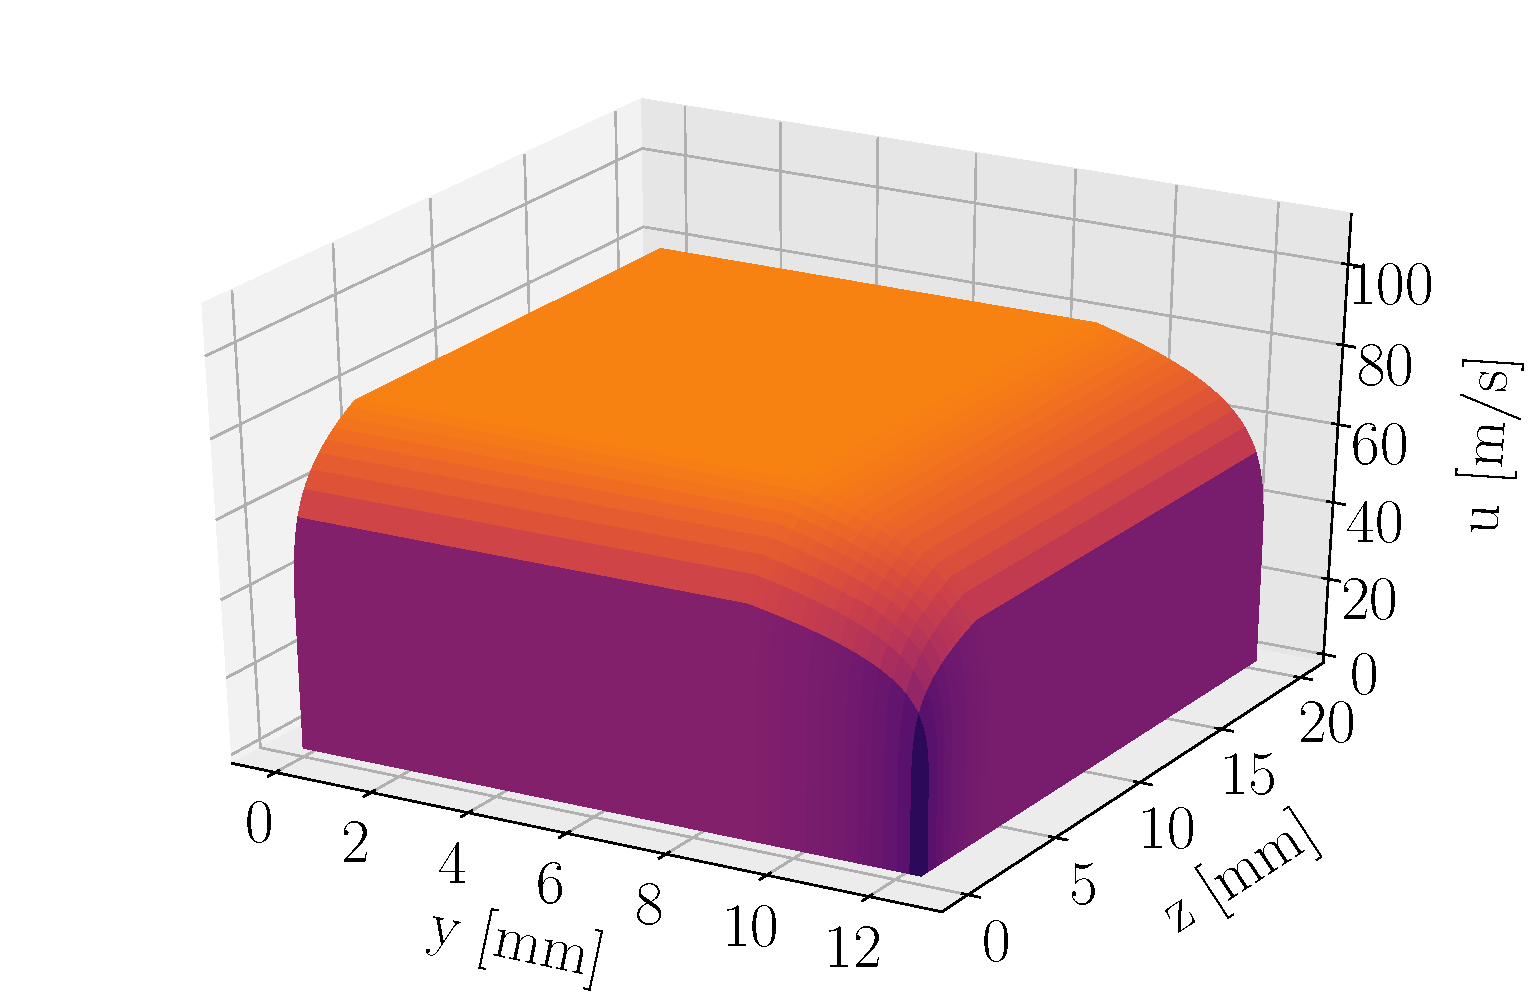
\includegraphics[scale=0.3]{./appendices_figures/gaseous_inlet_u_profile_75.eps}
     \end{subfigure}
     %\hfill
     \begin{subfigure}[b]{0.45\textwidth} 
         \centering
          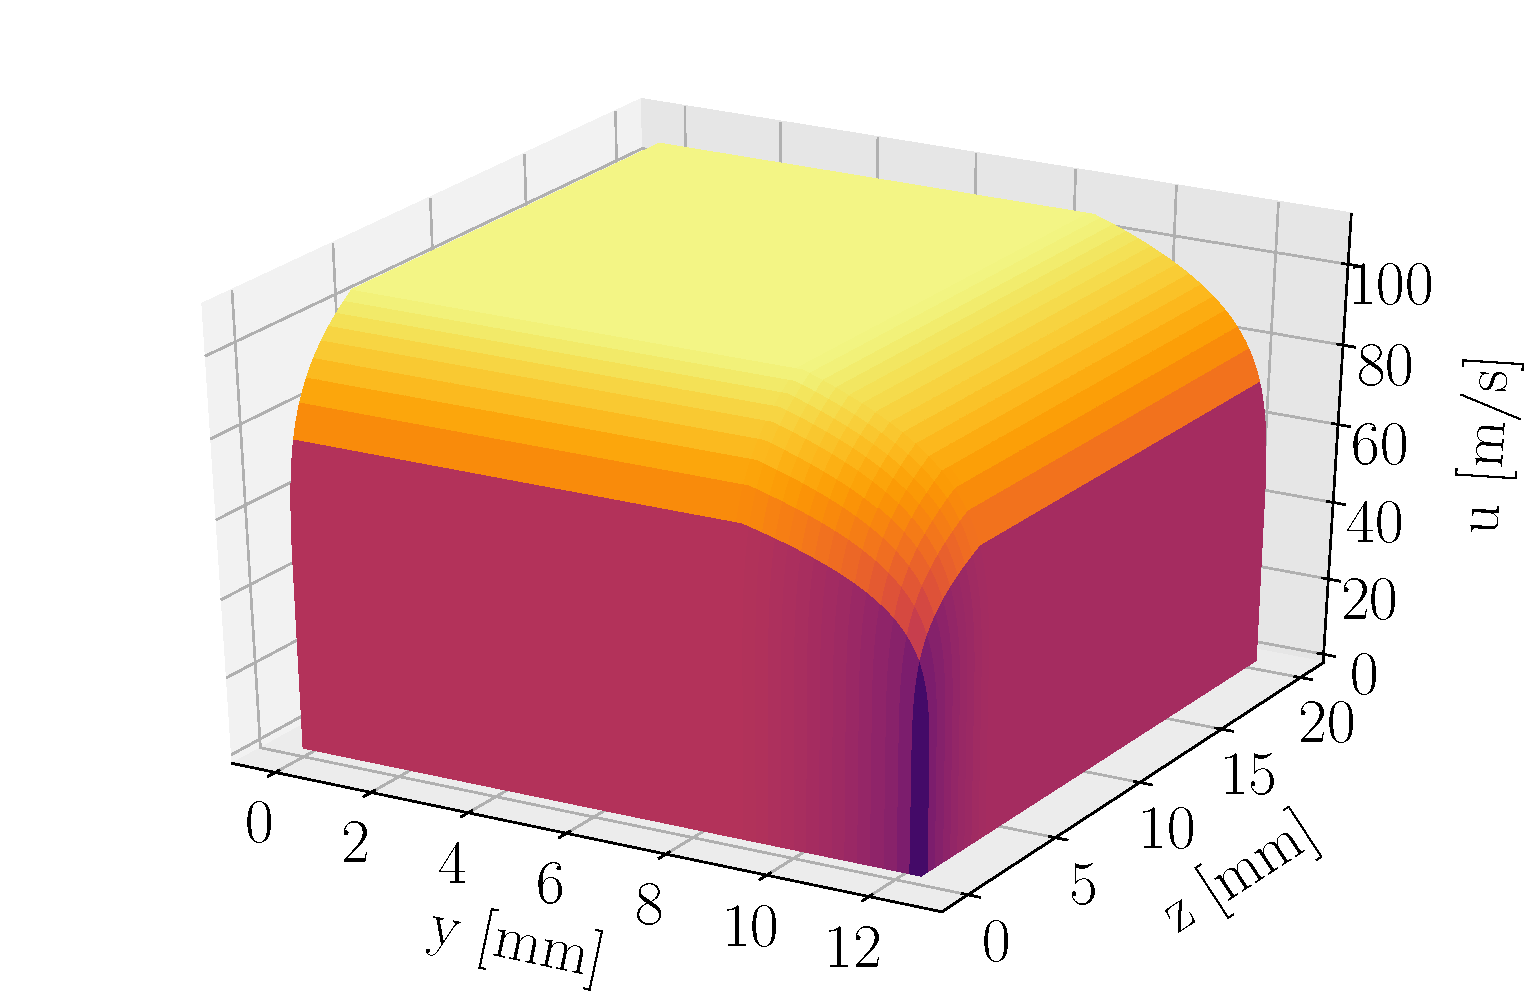
\includegraphics[scale=0.3]{./appendices_figures/gaseous_inlet_u_profile_100.eps}
     \end{subfigure}
        \caption[Gaseous inlet velocity profiles imposed]{Gaseous inlet velocity profiles imposed. One quarter of the domain is shown, the profile is then symmetric in both $y$ and $z$ axes. \textsl{Left}: $u_g = 75$ m $s^{-1}$. \textsl{Right}: $u_g = 100$ m $s^{-1}$.}
        \label{fig:resulting_velocity_profiles}
\end{figure}

